\documentclass{article}
\usepackage{fancyhdr}
\usepackage{ctex}
\usepackage{listings}
\usepackage[a4paper, body={18cm,22cm}]{geometry}
\usepackage{amsmath,amssymb,amstext,wasysym,enumerate,graphicx}
\usepackage{float,abstract,booktabs,indentfirst,amsmath}
\usepackage{multirow}
\usepackage{enumitem}
\usepackage{listings}
\usepackage{xcolor}
\usepackage{tabularx}
\usepackage[most]{tcolorbox}
\usepackage{accsupp}
\usepackage[bottom]{footmisc}
\usepackage{subcaption}
\usepackage{longtable}
% \usepackage[backend=biber,style=numeric]{biblatex}
\usepackage[xetex]{hyperref}
\usetikzlibrary{arrows.meta}
\newcommand\emptyaccsupp[1]{\BeginAccSupp{ActualText={}}#1\EndAccSupp{}}
\setlength{\parindent}{2em}
\renewcommand\arraystretch{1.4}
\setmonofont{Fira Code}
\setCJKmonofont{黑体}
% \setmainfont{Times New Roman}
\hypersetup{CJKbookmarks=true,colorlinks=true,citecolor=blue,%
            linkcolor=blue,urlcolor=blue,bookmarksnumbered=true,%
            bookmarksopen=true,breaklinks=true}
\lstset{
    % language = C,
    xleftmargin = 3em,xrightmargin = 3em, aboveskip = 1em,
	backgroundcolor = \color{white}, % 背景色
	basicstyle = \small\ttfamily, % 基本样式 + 小号字体
	rulesepcolor= \color{gray}, % 代码块边框颜色
	breaklines = true, % 代码过长则换行
	numbers = left, % 行号在左侧显示
	numberstyle = \small\emptyaccsupp, % 行号字体
    numbersep = 14pt, 
    keywordstyle=\color{purple}\bfseries, % 关键字颜色
    commentstyle =\color{red}, % 注释颜色
    stringstyle = \color{red}, % 字符串颜色
    morekeywords={ASSERT, int64_t, uint32_t},
	frame = single, 
	showspaces = false, % 不显示空格
    showstringspaces = false,
	columns = fixed, % 字间距固定
    literate=
        {^-}{{{\color{black}\textbf{\color{red}-}}\colorbox{red!30}{\phantom{XX}}}}{1}
        {^+}{{{\color{black}\textbf{\color{green}+}}\colorbox{green!30}{\phantom{XX}}}}{1},
}

\raggedbottom

\title{\textbf{大语言模型引导策略\ 实验与分析}}
\author{第七组 \\ 
李鹏达 10225101460 \\[-1em]
武泽恺 10225101429 \\[-1em]
张耘彪 10225101437
}
\date{}

\begin{document}
\maketitle

\section{简介}

在对大语言模型引导策略进行进一步修改后,我们再一次进行了初步的实验——对随机策略(random)、原有大语言模型引导策略(llm)和我们提出的大语言模型引导策略(new)三种策略在两个开源应用程序Ominotes和AnkiDroid上进行测试。我们使用覆盖率作为评估指标,并将测试结果与随即策略和原有大语言模型引导策略进行对比,以验证我们提出的新策略的有效性。

\section{实验环境}

\begin{itemize}[noitemsep]
    \item 操作系统:Windows 11 家庭中文版 26100.3915
    \item Python版本:3.11.9
    \item JaCoco版本:0.8.10
    \item Android Emulator版本:Pixel 9 API 34
\end{itemize}

\section{实验方法}

在实验中,我们使用JaCoco对安卓应用程序进行插桩,并使用Android Emulator进行测试。使用每个策略运行 Kea 至少120分钟或1200个事件,在测试过程中,每两分钟记录一次覆盖率数据。

实验结束后,分别根据运行时间和时间次数两个维度对覆盖率数据进行分析。我们将每个策略的覆盖率数据进行对比,并计算出每个策略的平均覆盖率和标准差。

我们的实验脚本可以在 \url{https://github.com/llipengda/kea-test} 中找到。

我们插桩的应用程序可以在 \url{https://drive.google.com/file/d/1XM7E4WIdaogFFO0z8kTrq3MsLTD-7pEp/view?usp=sharing} 下载。

\section{实验结果}

\begin{figure}[H]
\centering
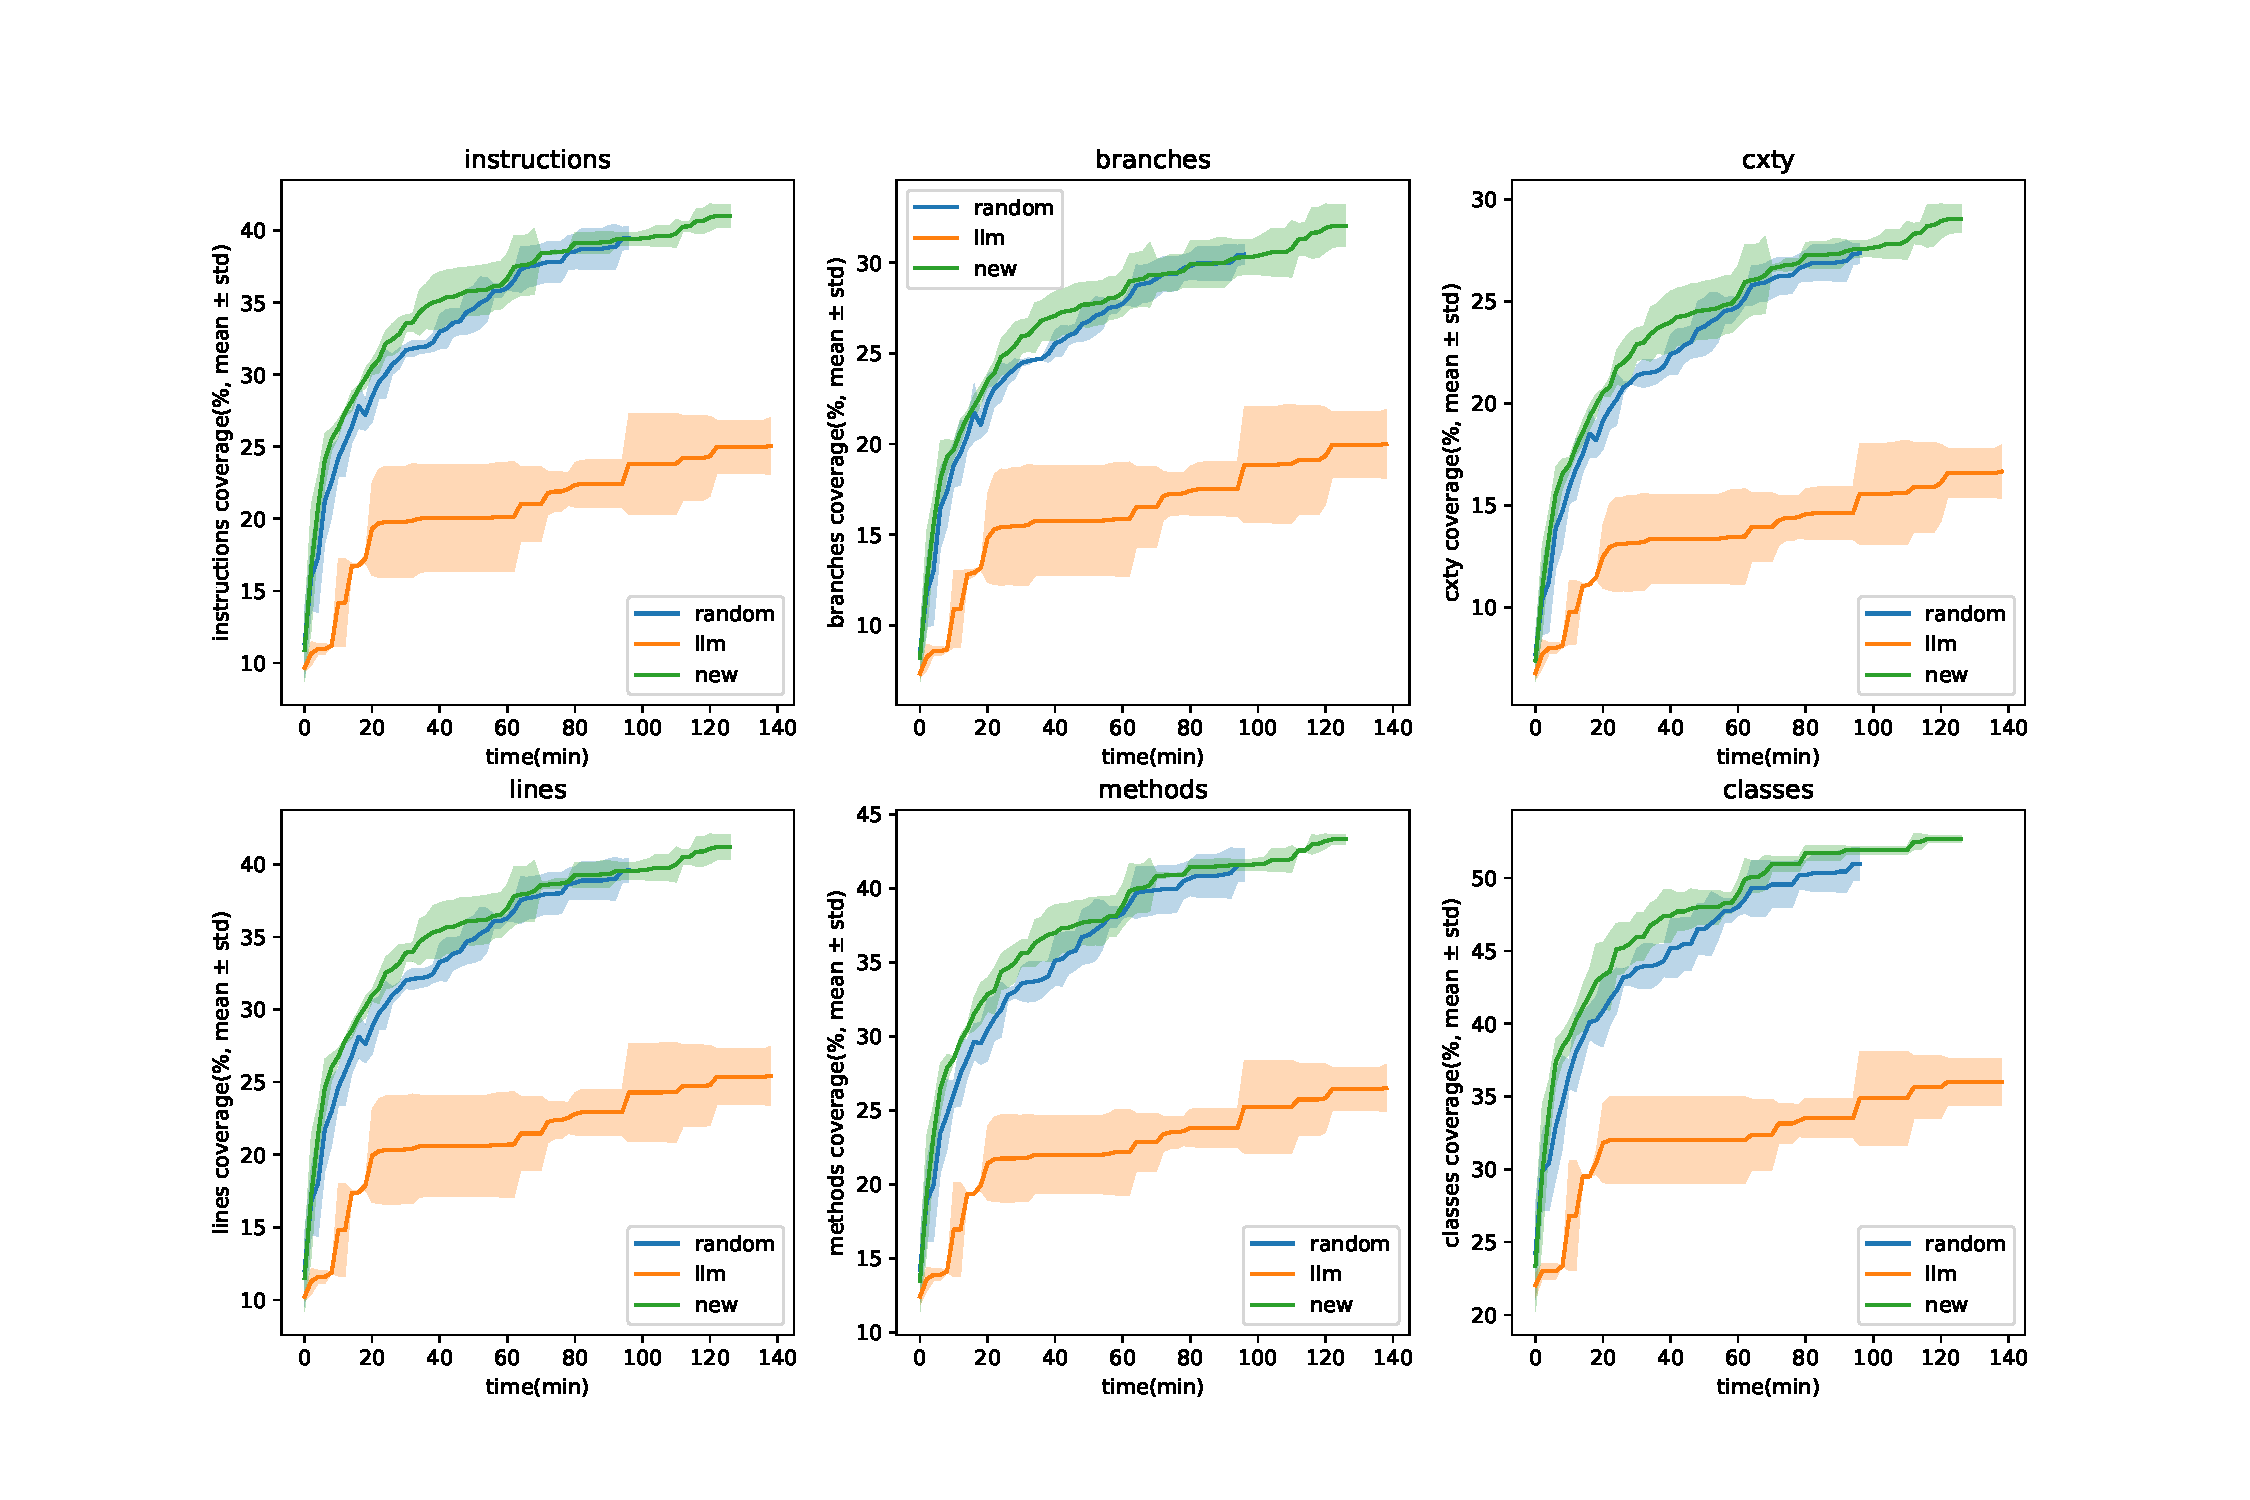
\includegraphics[width=\textwidth]{res/it.feio.android.omninotes.alpha/coverage_time.pdf}
\caption{OmniNotes覆盖率数据,按时间}
\end{figure}

\begin{figure}[H]
\centering
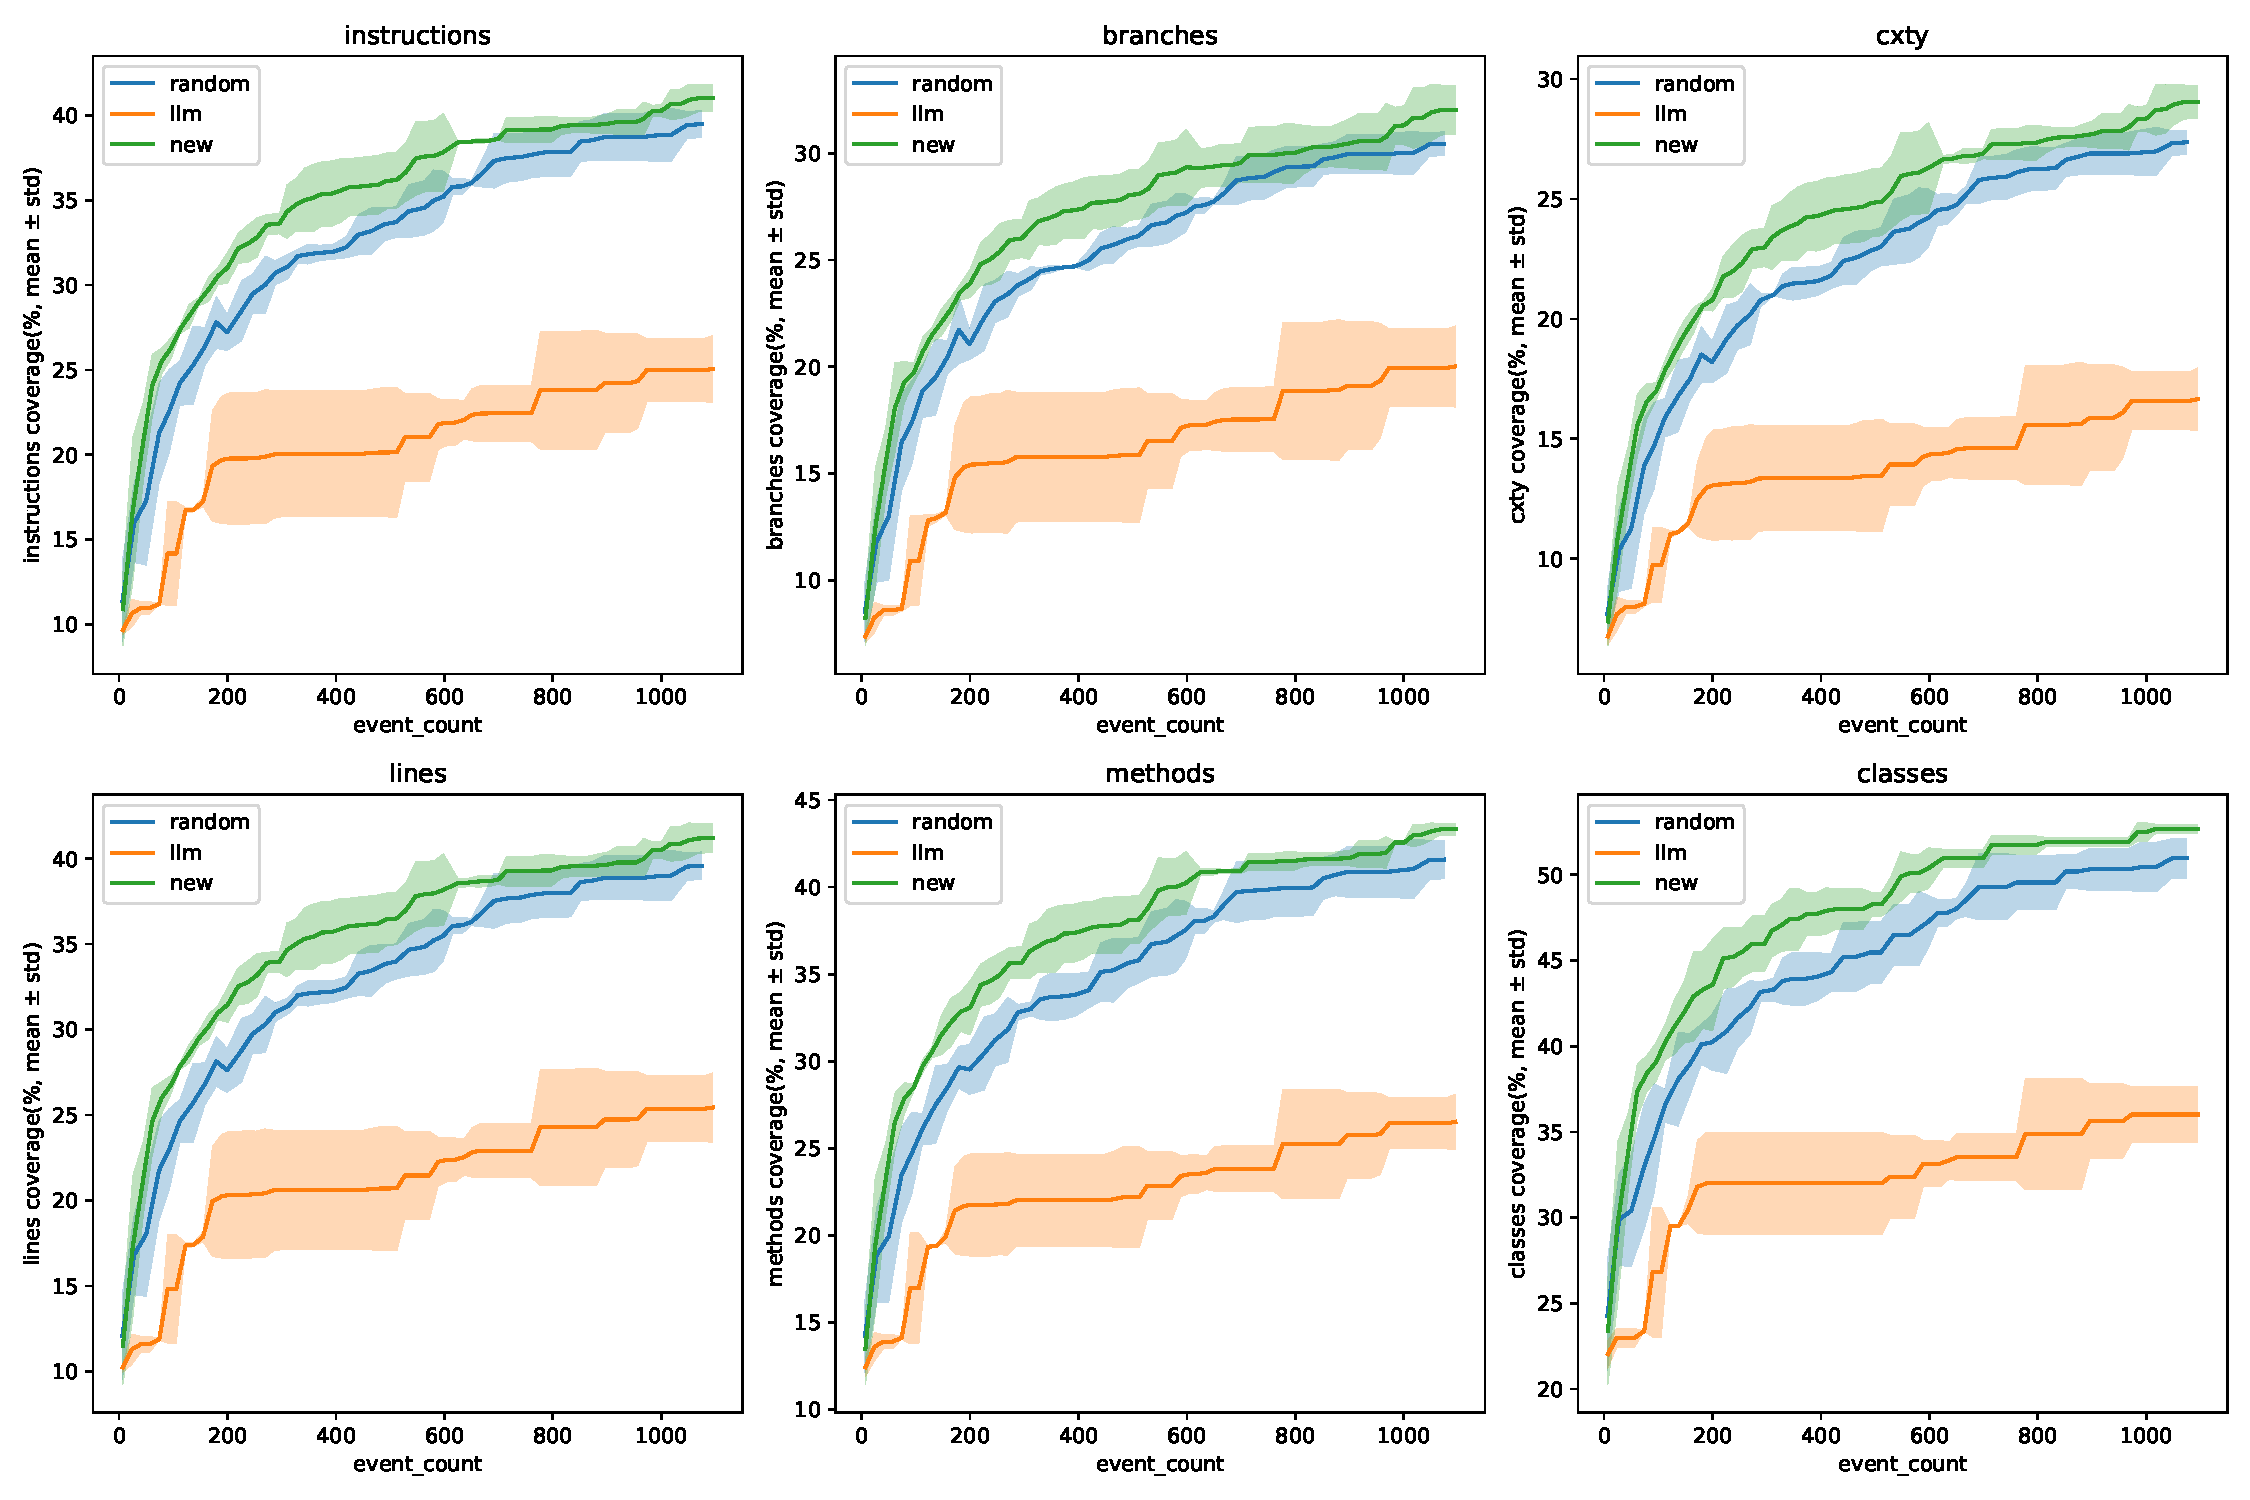
\includegraphics[width=\textwidth]{res/it.feio.android.omninotes.alpha/coverage_event.pdf}
\caption{OmniNotes覆盖率数据,按事件数}
\end{figure}

\begin{figure}[H]
\centering
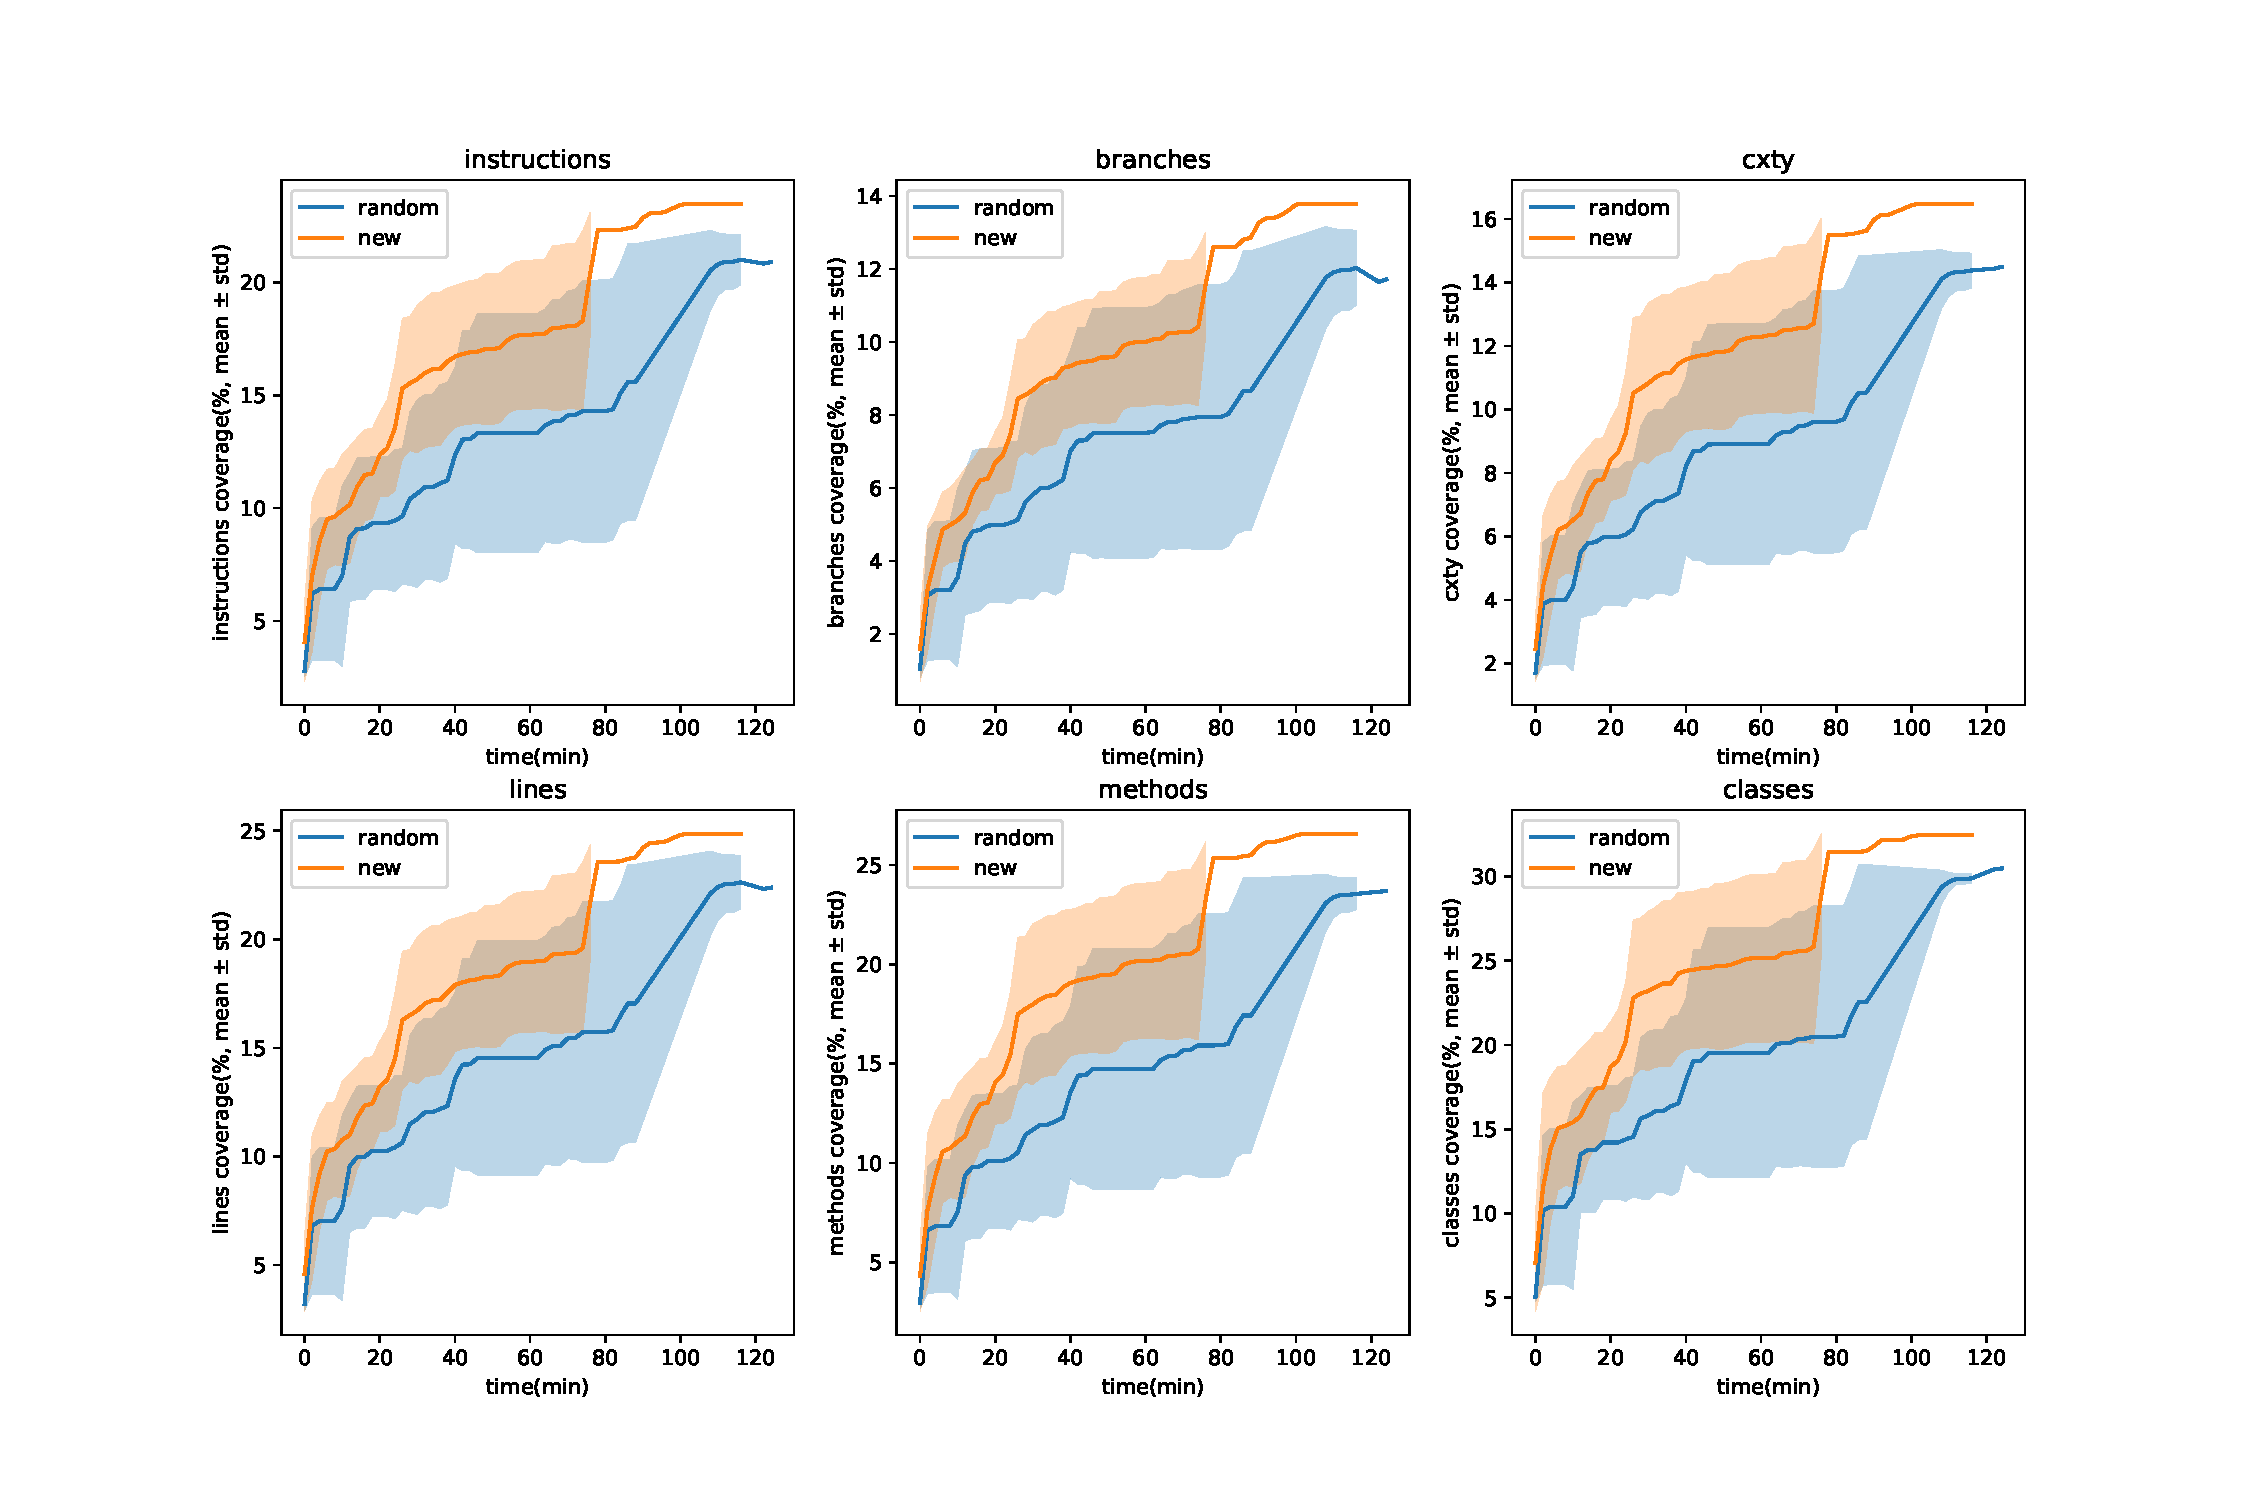
\includegraphics[width=\textwidth]{res/com.ichi2.anki.debug/coverage_time.pdf}
\caption{AnkiDroid覆盖率数据,按时间}
\end{figure}

\begin{figure}[H]
\centering
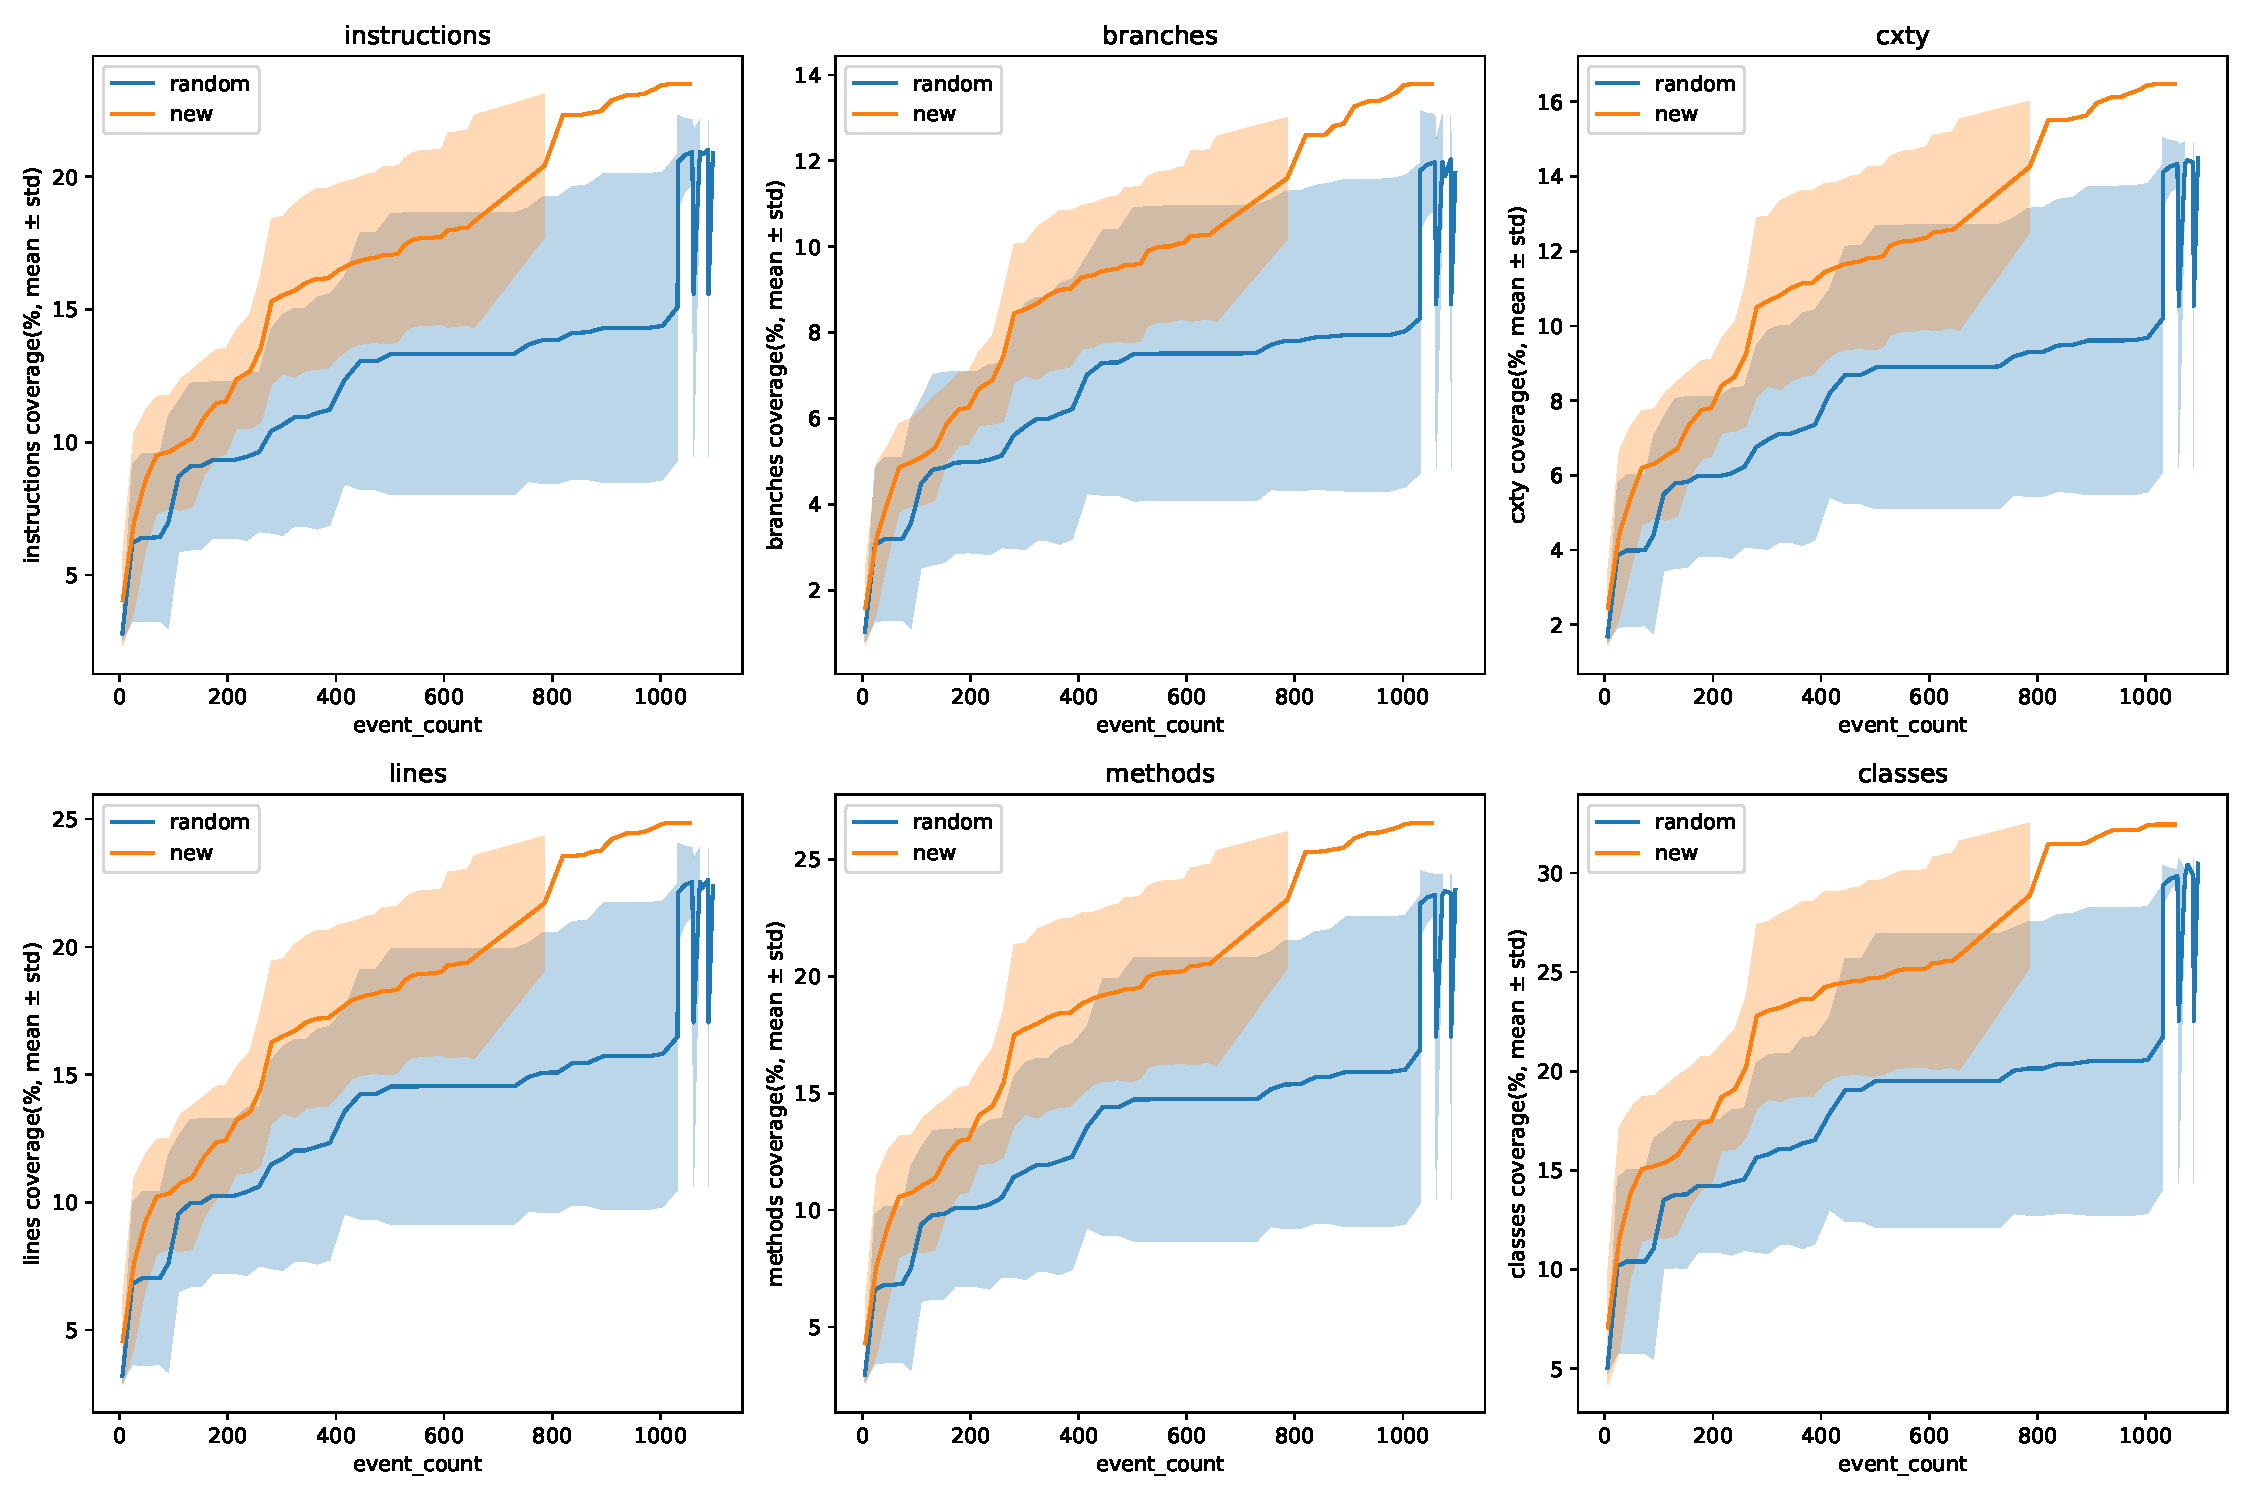
\includegraphics[width=\textwidth]{res/com.ichi2.anki.debug/coverage_event.pdf}
\caption{AnkiDroid覆盖率数据,按事件数}
\end{figure}

\section{实验分析}

实验数据表明,对于Ominotes应用程序,我们的策略覆盖率在时间维度上较随机策略略有提升,大幅优于原有大语言模型引导策略;在事件数维度上,我们的策略覆盖率较随机策略有一定提升,且提升大于时间维度,大幅优于原有大语言模型引导策略。这说明我们的策略在运行相同事件时能够得到更高的覆盖度。但由于引入了大语言模型,导致运行速度有所下降,因此在时间维度提升不明显。查。

而对于AnkiDroid应用程序,无论是在时间维度还是事件次数维度,我们的策略均对于随机策略有明显的提升。经过对实验数据的分析,我们猜测这可能是由于这该应用程序中含有WebView和登录页面,导致随机策略更容易陷入UI陷阱。

值得注意的是,无论是哪个应用程序,哪种策略,得到的覆盖度都是比较低的,而且观察可以发现它们均有大量的页面没有探索。

\end{document}